\paragraph{\cx{Forecast model choice.}}\label{sec:forecast_utility}
\cx{To forecast one neuron's activity, we need to choose a model from the observations so far. Testing every candidate on earlier parts of the record takes time. We ask whether MG of the observed activity can guide the choice. Figure~\ref{fig:single-neuron-forecasts} shows cases where MG and held-out search choose different models. The two selection methods yield similar mean forecast errors, with substantial uncertainty about the gap (Table~\ref{tab:forecast_all}).}

\cx{Computing MG at a subset of delay vectors preserves every model choice in this evaluation and reduces selection time below held-out search on the same inputs (Table~\ref{tab:forecast_utility}).}

\begin{table}[htbp]
\centering\small
\caption{\cx{Forecast error and selection time. NMSE uses prefix variance and is mean $\pm$ SD across 20 repeats after averaging tasks within each repeat. Time is the median on matched inputs.}}
\label{tab:forecast_utility}
\begin{tabularx}{\linewidth}{@{}>{\raggedright\arraybackslash}Xrr@{}}
\toprule
Selection rule & NMSE & Time (ms) \\
\midrule
MG, all queries (KD-tree) & $0.0364\,\pm 0.0213$ & 199.1 \\
\cx{MG, 128 queries (direct distance calculation)} & $0.0364\,\pm 0.0213$ & 12.2 \\
Lowest validation error & $0.0407\,\pm 0.0324$ & 45.3 \\
\bottomrule
\end{tabularx}

\end{table}

\begin{figure*}[htbp]
\centering
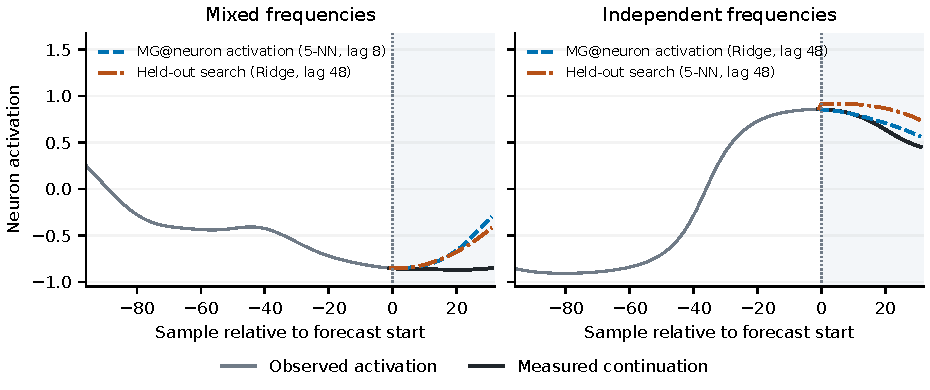
\includegraphics[width=.96\textwidth]{figures/single_neuron_forecasts.pdf}
\caption{\cx{Forecasts from the same held-out repeat. The plots show the end of the observed prefix. Held-out search is closer on the mixed-frequency target, and MG selects the closer forecast on the independent-frequency target.}}
\label{fig:single-neuron-forecasts}
\end{figure*}
